% Template created by Karol Kozioł (www.karol-koziol.net) for ShareLaTeX

\documentclass[a4paper,9pt]{extarticle}
\usepackage[utf8]{inputenc}
\usepackage[T1]{fontenc}

\usepackage{graphicx}
\graphicspath{ {images/} }

\usepackage{xcolor}
\usepackage{tikz}

\usepackage{amsmath,amssymb,textcomp}
\everymath{\displaystyle}

\usepackage{times}
\renewcommand\familydefault{\sfdefault}
\usepackage{tgheros}
\usepackage[defaultmono,scale=0.85]{droidmono}

\usepackage{multicol, caption}
\setlength{\columnseprule}{0pt}
\setlength{\columnsep}{20.0pt}


\usepackage{geometry}
\geometry{
a4paper,
total={210mm,297mm},
left=10mm,right=10mm,top=10mm,bottom=15mm}

\linespread{1.3}


% custom title
\makeatletter
\renewcommand*{\maketitle}{%
\noindent
\begin{minipage}{1\textwidth}

\begin{tikzpicture}
\node[rectangle,rounded corners=6pt,inner sep=10pt,fill=blue!50!black,text width= 0.95\textwidth] {\color{white}\Huge \@title};
\end{tikzpicture}
\end{minipage}
\bigskip\bigskip
}%
\makeatother

% custom section
\usepackage[explicit]{titlesec}
\newcommand*\sectionlabel{}
\titleformat{\section}
  {\gdef\sectionlabel{}
   \normalfont\sffamily\Large\bfseries\scshape}
  {\gdef\sectionlabel{\thesection\ }}{0pt}
  {
\noindent
\begin{tikzpicture}
\node[rectangle,rounded corners=3pt,inner sep=4pt,fill=blue!50!black,text width= 0.95\columnwidth] {\color{white}\sectionlabel#1};
\end{tikzpicture}
  }
\titlespacing*{\section}{0pt}{15pt}{10pt}


% custom footer
\usepackage{fancyhdr}
\makeatletter
\pagestyle{fancy}
\fancyhead{}
\fancyfoot[C]{\footnotesize \textcopyright\ \@date\ \ \@author}
\renewcommand{\headrulewidth}{0pt}
\renewcommand{\footrulewidth}{0pt}
\makeatother

\newenvironment{Figure}
  {\par\medskip\noindent\minipage{\linewidth}}
  {\endminipage\par\medskip}


\title{Fundamentos de Algoritmos y computabildad}



\begin{document}

\maketitle

\begin{multicols*}{2}


\section{Conceptos fundamentales}

\subsection{Problemas en la computabilidad}

\subsubsection{Decibilidad} ¿Que puede hacer una computadora?
\subsubsection{Intrabilidad} ¿Que puede hacer una computadora eficientemente?


\subsection{Alfabeto} 
Un alfabeto \( \Sigma \) es un conjunto de símbolos finito y no vacío. 

\begin{itemize}
\item $( \Sigma ) = (0, 1)$ El alfabeto de los números binarios.
\end{itemize}

\subsubsection{Potenciación de Alfabetos}
Definimos $\Sigma^k$ como el conjunto de cadenas de longitud $k$, tales que cada uno de los simbolos pertenece a  $\Sigma$

Si $\Sigma = (0, 1)$
\begin{itemize}
\item $\Sigma^0 = \{\epsilon\}$
\item $\Sigma^1 = \{0, 1\}$
\item $\Sigma^2 = \{00, 01, 10, 11\}$
\item $\Sigma^* =$ Todas las cadenas del alfabeto
\end{itemize}

\subsection{Cadena, Cadena de caracteres o Palabra}
Secuencia finita de simbolos seleccionados de un alfabeto.

\subsubsection{Cadena vacia}
La cadena vacia es la cadena sin simbolos y se denomina $\epsilon$.

\subsubsection{Concatenación}
La concatención de cadenas $x,y$ se define como la cadena formada por una copia $x$ seguida por una copia de $y$.

\subsection{Lenguajes}
Un conjunto de cadenas seleccionadas de un alfabeto se conocen como lenguaje. Algunos ejemplos de lenguajes son el español, o el lenguaje Java. Es pósible expresar los lenguajes mediante la descripción de conjuntos.

\begin{itemize}
\item \{w | w consta de un número igual de ceros que de unos\}
\item \{ $0^n1^n | n \geqslant 1$  \}. El conjunto de 0 a la n, 1 a la n talque n es mayor o igual que 1.
\end{itemize}


\section{Desmostraciones}
\begin{description}
\item[Deductivas] Listas de proposiciones verdaderas o que se deducen lógicamente de las proposiciones anteriores.
\item[Si-entonces] Se parte de una hipótesis y se llega a la validación de la tesis.
\item[Si y sólo si] Se demuestran porbando que cada conjunto está contenido en el otro.
\item[Reducción a lo absurdo] Consiste en negar la hipótesis y llegar a un absurdo.
\item[Demostración inductiva] Consiste primero en demostrar un caso base, después extender la demostración a un número finito de casos hasta n, luego se demuestra  
\item[Contra-ejemplo] Es útil para demostrar la falsedad de una proposición la idea es proporcionar un contraejemplo que hace la proposición falsa.
\end{description}

\section{Autómatas}

\subsection{Autómatas finito determinista}
Un autómata finito determinista consta de: $M = \{Q, \Sigma, \delta, q_o, F\}$

\begin{enumerate}
\item Un conjunto finito de estados $Q$
\item Un conjunto finito de símbolos de entrada $\Sigma$
\item Una función de transición $\delta$ que toma como argumentos un estado y un símbolo de entrada y devuelve un estado.
\item Un estado inicial $q_0$
\item un conjunto de estados finales $F$.
\end{enumerate}

\begin{Figure}
 \centering
 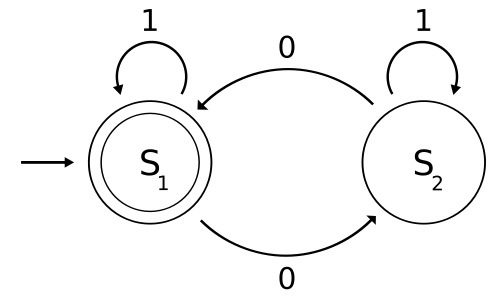
\includegraphics[scale=0.3]{AFD}
 \captionof{figure}{Representación de un autómata}
\end{Figure}



\subsubsection{Lenguaje de un AFD}
Se denomina el lenguaje de un AFDA $(Q, \Sigma, \delta, q_0, F)$ como:

$L(A) = \{w| \delta(q_0, w)$ pertenece a F \}

\subsection{Autómatas finitos no deterministas (AFN)}
Un autómata finito "no  determinista tiene la capacidad de estar en varios estados a la vez. La principal diferente es que la función de transacción $\delta$ devuelve un subconjunto de estados.

\subsubsection{Lenguaje de un AFD}
Se denomina el lenguaje de un AFN como el conjunto de cadenas de $w$ pertenecientes a $\Sigma_*$ tal que $\delta(q_0, w)$ contiene al menos un estado de aceptación.

\subsubsection{Función transferencia AFD vs AFN}
\begin{description}
\item[AFD] $Q X \Sigma \longrightarrow Q$ donde |Q| = 1
\item[AFD] $Q X \Sigma \longrightarrow 2^Q$ donde $2_Q$ es el power set de Q
\end{description}

\subsubsection{Equivalencia entra AFN y AFD}
Para demostrar que \textit{L(D)=L(N)} dado un AFN $\{Q_N, \Sigma, \delta_N, Q_0, F_N \}$ y un AFD $\{Q_D, \Sigma, \delta_D, \{Q_0\}, F_D \}$

\begin{enumerate}
\item $Q_d$ es el conjunto de subconjuntos de $Q_N$. $Q_d$ tendrá a lo máximo $2^n$ estados.
\item $F_D$ es el conjunto de subconjuntos que incluyen al menos un estado de aceptación $F_D$.  $F_D$ es el conjunto de subconjuntos S de $Q_N$ tal que $S \cap F_N \neq \phi $
\item Para cada $S \subseteq Q_N$ y para cada símbolo de entrada a perteneciente a $\Sigma$
\end{enumerate}

\subsection{Conversión AFN - AFD}

\begin{Figure}
 \centering
 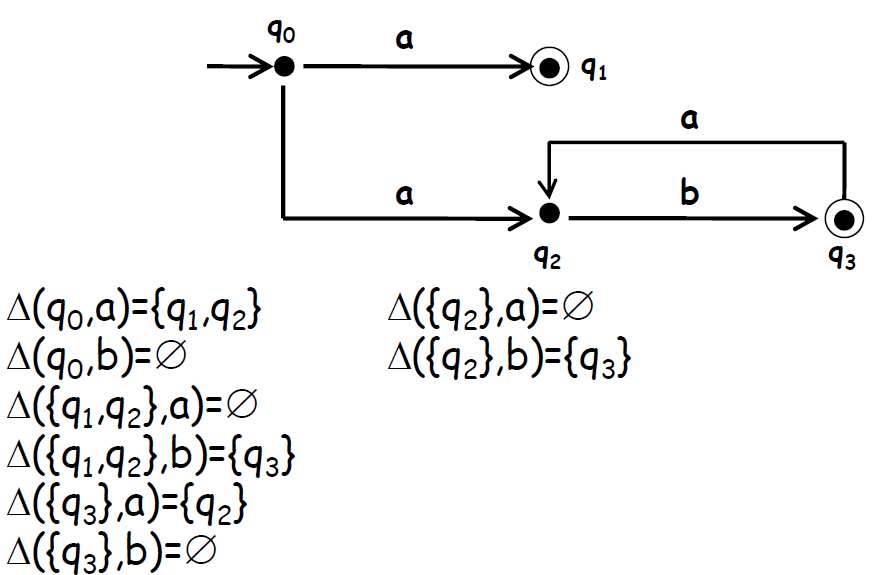
\includegraphics[scale=0.3]{AFN_AFD}
 \captionof{figure}{Conversión AFN - AFD. Lista de transiciones}
\end{Figure}

\begin{Figure}
 \centering
 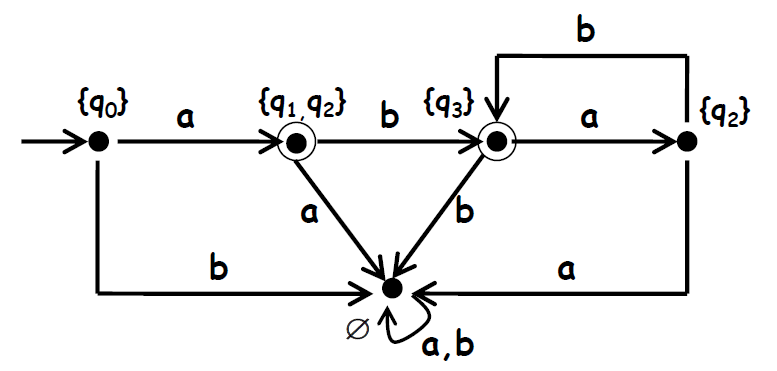
\includegraphics[scale=0.3]{AFN_equivalente}
 \captionof{figure}{Conversión AFN - AFD. AFN equivalente}
\end{Figure}


\subsection{Autómatas finitos con transiciones-$\epsilon$}
Las transición $\epsilon$ son transiciones con la cadena vacía, esto significa que un AFN puede hacer una transición  espontánea sin recibir un símbolo de entrada.

\begin{Figure}
 \centering
 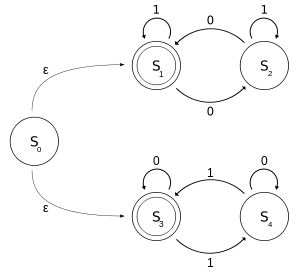
\includegraphics[scale=0.5]{AFNE}
 \captionof{figure}{Representación de un autómata no determinista con transiciones epsilon}
\end{Figure}

\subsection{Estado muerto}
Un estado muerto es aquel que al entrar la computación del autómata va a estar confinada a ese estado hasta la finalización de la cadena de entrada.

\begin{Figure}
 \centering
 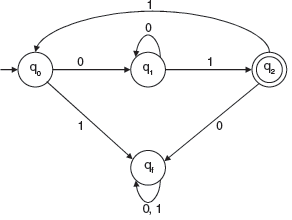
\includegraphics[scale=0.7]{dead_state}
 \captionof{figure}{El estado $q_f$ representa un estado muerto}
\end{Figure}

\subsection{$\epsilon$ - cerradura de q}

\begin{itemize}
\item $e-c(q)=$ \{p|p es un estado accesible desde q sin consumir ningún símbolo\}
\item $d(\epsilon - c(1), \sigma)$ es el conjunto de estados accesibles desde q, tomando primero una o más $\epsilon$-transiciones y luego una transición con $\sigma$.
\item $\epsilon - c(d(\epsilon - c(1), \sigma))$, es el conjunto de estados accesibles desde q, tomando primero una o más $\epsilon$-transiciones, luego una transición con $\sigma$ y luego una o más $\epsilon$-transiciones.
\end{itemize}


\subsection{Eliminación de estados épsilon $\epsilon$}

\begin{Figure}
 \centering
 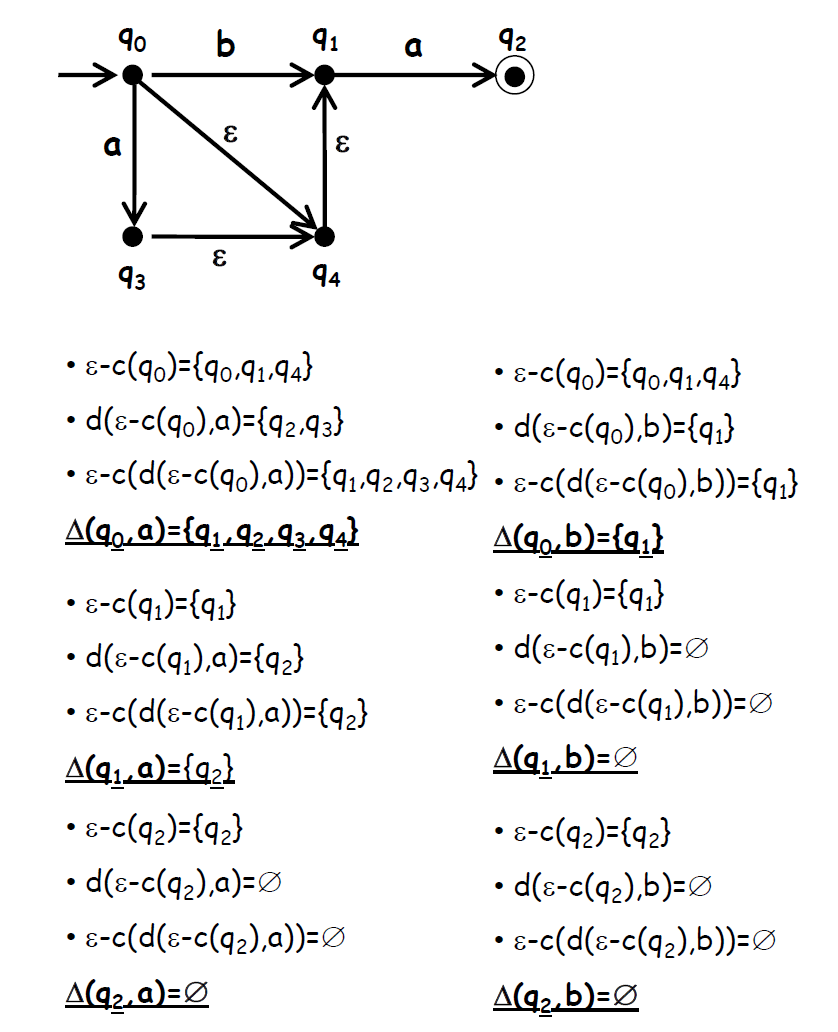
\includegraphics[scale=0.4]{Eliminar_epsilon}
 \captionof{figure}{Proceso para remover transiciones épsilon}
\end{Figure}

Finalmente se crea un AFND que puede ser reducido a un AFD

\begin{Figure}
 \centering
 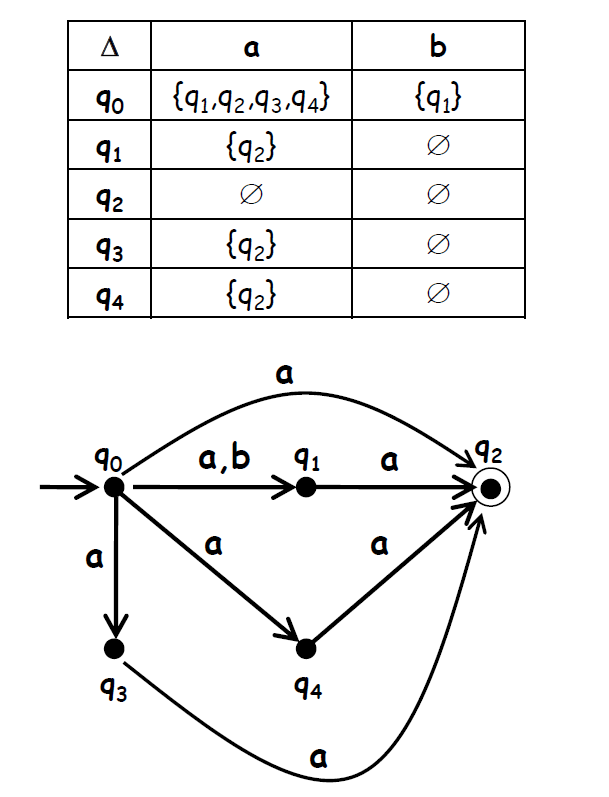
\includegraphics[scale=0.4]{Eliminar_epsilon_resultado}
 \captionof{figure}{Resultado de la eliminación de transiciones épsilon}
\end{Figure}



\section{Expresiones regulares}
Una expresión regular es el lenguaje que puede ser procesado por un autómata. Por su naturaleza declarativa son útiles para expresar las cadenas que se pueden aceptar.

\subsection{Teorema de Kleene}
Un lenguaje es regular si y sólo si es aceptado por un autómata finito.

\subsection{Operadores de las expresiones regulares}
\begin{description}
\item[Unión] $L = {001, 10, 111}$ y $M = \{\epsilon, 001\}$, entonces $L  \cup M=\{\epsilon, 10, 001, 11\}$
\item[Concatenación] $L = {001, 10, 111}$ y $M = \{\epsilon, 001\}$, entonces $LM=\{001, 10, 111, 001001, 10001, 111001 \}$
\item[Clausura de Kleene $L^*$] Es el conjunto de cadenas que se pueden formar tomando cualquier número de cadenas de L.
\end{description}

\subsection{Autómatas finitos y expresiones regulares}
Las expresiones regulares son la notación algebraica  para representan los mismos lenguajes que los autómatas.

\subsection{AFD a expresión regular}

\subsection{Expresión regular a AFD}

\subsection{Álgebra de las expresiones regulares}
\begin{description}
\item[Conmutativa de la unión] $L+M=M+L$
\item[Asociativa por la unión] $(L+M)+N = L + (N +M)$
\item[Asociativa por la concatenación] $(LM)N = L(MN)$
\item[Distributiva por la izquierda] $L(M +N) = LM - LN$
\item[Distributiva por la derecha] $(M + N)L = ML + NL$
\item[Idempotencia para la unión] $L+L = L$
\item[Clausuras] $(L^*)^* = L^* $, $ \theta ^* = \epsilon$, $\epsilon^*=\epsilon$, $L^+=LL^*$
\end{description}


\subsection{Lema de Arden}
Una ecuación de la forma $X=AX \cup B$, donde A, B, X son lenguajes y $\epsilon \notin A $(A no contiene la cadena vacía), tiene una solución única $X=A*B$, $X=A*B$

\subsection{El Lema de bombeo}
Sea L un lenguaje regular. Existe entonces una constante n tal que para todo w perteneciente a L con $|w| \geq n$, podemos descomponer w en tres cadenas $xyz$ tales que:

\begin{enumerate}
\item $y \neq \epsilon $
\item $|xy| \leq n$
\item Para todo $k \geq 0$, la cadena $xy^kz$ tambien pertenece a L.
\end{enumerate}

\section{Gramáticas independientes del contexto}
Una gramática independiente del contexto esta definida por sus 4 componentes:

\begin{enumerate}
\item Un conjunto de símbolos que forma las cadenas del lenguaje
\item Un conjunto finito de variables. Cada variable representa un lenguaje.
\item Un símbolo inicial.
\item Un conjunto finito de producciones o reglas que representan la definición recursiva del lenguaje de la forma $variable \longrightarrow variable + simbolos$
\end{enumerate}

\subsection{Lenguaje de una gramática}
Dada una gramática $G(N, T, P, S)$ el lenguaje G es el conjunto de las cadenas terminales que tienen derivaciones desde el símbolo inicial S.

\subsection{Gramáticas ambiguas}
Se dice que una gramática es ambigua si para la generación de una cadena mas de una árbol de expresiones puede ser generado.

\subsection{Simplificación de una gramática independiente del contexto}
Una gramatica puede ser simplicada al

\begin{enumerate}
\item Remover símbolos que no generan símbolos terminales
\item Remover símbolos no alcanzables
\item Eliminar las producciones de renombramiento. 
\item Eliminar las producciones nulas.
\end{enumerate}


\subsection{Forma normal de Chomsky}
Un gramática esta en la forma normal de Chomsky si sus reglas de producción son de la forma.

\begin{itemize}
\item $A \longrightarrow BC$
\item $A \longrightarrow a$
\end{itemize}

Donde $ABC$ son símbolos no terminales y $a$ es un símbolo terminal. 

\subsection{Forma normal de Greibach}
Una gramática esta en formal normal de Greibach si:

\begin{enumerate}
\item la variable inicial no es recursiva.
\item no tiene variables inútiles.
\item no tiene producciones $\lambda$ (excepto posiblemente $S \longrightarrow \lambda$).
\item sus producciones son de la forma $A \longrightarrow \alpha$ es decir producciones simples o $A \longrightarrow aB_1, B_2 ... B$ donde $B_i$ son variables.
\end{enumerate}{}

\subsection{Lema del bombeo para gramáticas independientes del contexto}

Dado un lenguaje L independiente del contexto. Es posible encontrar un número natural n que.

\begin{enumerate}
\item para cada $ z \in L $ con $z \geq n$ puede ser escrito como w = uvwxy para cadenas u,v,w,x,y
\item $|vx| \geq$ 1
\item $|vwx| \leq n $
\item $uv^k wx^k y \in L$ para todo $k \geq 0$
\end{enumerate}


\end{multicols*}

\end{document}
